\section{Broader impacts}\label{sec:broader}
This paper presents methods to train LLMs more efficiently:
practitioners can use our methods to reduce the total compute FLOPs
used to train models, subject to time constraints.
%
Given the intense pressure to advance LLM capabilities as quickly as
possible, our methods can therefore reduce the associated
environmental and financial costs of LLM
training~\citep{patterson2021carbon,bender2021dangers}.

Moreover, hyperparameter tuning is a key contributor to these costs,
and impairs equity in AI research, as tuning success depends directly
on researcher finances~\citep{strubell2019energy}.
% For models that will be re-trained, \emph{sensitivity} to
% hyperparameters also leads to downstream
% costs~\citep{strubell2019energy}.
We hope our exploration of optimal hyperparameter scaling can reduce
the burden of hyperparameter tuning at scale and thus improve equity
in AI\@.


\section{Limitations}\label{sec:limitations}
While our findings corroborate prior work and provide strong evidence
for the proposed scaling laws in $\tepoch$, $\bopt$, and $\bcrit$,
there are several limitations that merit further study.

\paragraph{EMA perspective}

As the EMA perspective regards parameters $y_t$ as a function of
updates $x_t$, it fails to account for $x_t$ actually depending on
earlier values of $y_t$ (e.g., $y_{t-1}$). Yet although this
perspective has formal limitations, we nevertheless find it a
useful \emph{conceptual} model of training, as it predicts behavior
that is supported by experiments.

\paragraph{Optimization and training setup}

Our work focuses on AdamW (the standard optimizer for LLM training).
While the EMA perspective applies directly to other optimizers that
use decoupled weight decay, such as Sophia~\citep{liu2023sophia} and
MuonClip~\citep{kimi2025k2}, it may not apply to approximate second
order methods, e.g., Shampoo~\citep{gupta2018shampoo}.  However, it
can be used when applying AdamW (and related optimizers) in Shampoo's
eigenbasis, which was shown to be effective in
SOAP~\citep{vyas2024soap}.

We present results with a single (standard) learning rate schedule.
Our method for obtaining $\cbs$ estimates would be quite efficient
with a warmup-stable-decay (WSD)
schedule~\citep{hu2024minicpm,wen2024understanding}, as we could
perform a single training run with each batch size, but decay at
various milestones in order to get points along the scaling law,
essentially following the approach in~\citet{hagele2024scaling}, but
with separate laws for each batch size.

We used the maximal update parameterization in all experiments, which
generates a learning rate $\eta$ adjustment for each model width.  Our
results suggest this approach enables good models at arbitrary $N$,
$D$, and $B$ when combined with adjustments to $\lambda$.  This
strategy is informed by our experiments comparing re-adjusting $\eta$
vs.\ $\lambda$ in \cref{sec:tema_results}. However, it is not
feasible, at this scale, to verify whether substantially better models
could be obtained by sweeping the full cross-product of $\eta$ and
$\lambda$ values.

Our study specifically focuses on the practically important setting of
single-epoch LLM pre-training.  \citet{wang2024how} indeed noted
differences in optimal $\tema$ when using multi-epoch training,
possibly due to data repetition. Reconciling these differences by
isolating the effects of repetition versus scale is an interesting
follow-up direction.

Here we only experimented with a single dataset, vocabulary, and
context length.  We obtained a similar $\cbs$ scaling law
to \citet{zhang2024how}, but it would be interesting to see if
differences in the coefficient of our power laws could be attributed
to specific differences in approach (e.g., differences in dataset,
context length, learning rate schedule, use of weight decay,
etc.).  \cref{sec:appendix_zhang} has further discussion of
differences with \citet{zhang2024how}.

We have also not explored how changes in numerical precision could
affect scaling laws.  Recent work~\citep{kumar2024scaling} showed
that, in terms of scaling laws, lower precision reduces the model's
\emph{effective} parameter count.  This suggests precision would
have no impact on scaling of $\bopt$ or $\bcrit$, which do not scale
in $N$.  Lower precision, however, could increase the \emph{effective}
TPP (via smaller effective $N$), thereby altering $\temaopt$.

\paragraph{Small batches, large batches, and dynamic batch sizing}

We consistently find that smaller and smaller batches do not grow
asymptotically closer to $\dmin$, as predicted by theory, but
eventually degrade in loss.  One possibility is that $\lambda$ tuning
is not sufficient with very small $B$, and further tuning of other
hyperparameters may be needed, such as the Adam $\beta$ parameters (as
suggested in recent
work~\citep{porian2024resolving,zhang2024how,marek2025small}).
%
Some preliminary tests using the $\beta_2$ scaling rule
from \citet{marek2025small} showed loss improvements at small $B$.
%
Since we are unlikely to train with small batches at scale, and using
them even with smaller LLMs significantly impairs our ability to train
both efficiently and quickly, it is unfortunately difficult to justify
further exploration in this direction.

Regarding large batches, our methods do not account for the many
practical systems-related issues, including bandwidth and
communication overheads, memory limits of hardware, synchronization
delays, etc.  
%
Moreover, as batch sizes increase, techniques such as optimizer
sharding may be needed, which further complicate performance
model~\citep{almazrouei2023falcon}.
%
Our scaling laws do, however, explicitly define a practically relevant
regime of training batch sizes: $\bopt \le
B \le \bcrit$. Practitioners can leverage this identified regime
alongside system-specific profiling (e.g., evaluating utilization at
various batch sizes) to select optimal settings balancing algorithmic
and systems constraints.

Exploring optimal dynamic batch sizing is a natural future direction
for our work.  While the potential gains were found to be small in
theory by \citet{mccandlish2018empirical}, more recent work has found
significant wall clock speedups~\citep{meterez2025seesaw}.
%
%We also plan to explore dynamic measurement of the gradient noise
%scale~\citep{mccandlish2018empirical}, which has been shown to be
%correlated with the empirical $\cbs$, and may thus help guide a
%dynamic batch size schedule.

%- We also only consider training TIME and training COMPUTE, rather
%than inference TIME and inference COMPUTE.
%
%- overtrained models do take more training compute but reduce
%inference time and compute~\citep{touvron2023llama}, but we note we
%provide nuance to this idea by noting smaller can also reduce training
%TIME both because they use less time per optimization steps, and
%because they allow greater parallelism through a larger batch size.
%
%- Ideally, if we had an idea of our total expected training compute +
%inference compute needs, we could add inference compute to the y-axis
%on our Pareto plots and compare against training time, perhaps also
%incorporating any constraints we have on inference time.


\section{Experimental Details}\label{sec:experimental_details}

\begin{table}
  \centering
  \caption{Model architectures used in experiments\label{tab:model_info}}
\begin{tabular}{@{}ccccc@{}}
\toprule
Model & $d_{model}$ & $n_{layers}$ & $d_{head}$ \\ \midrule
111M  & 768    & 10      & 64           \\
266M  & 768    & 32      & 64           \\
610M  & 2048   & 10      & 64           \\
1.7B  & 2048   & 32      & 64           \\
3.3B  & 2048   & 64      & 64           \\ \bottomrule
\end{tabular}
\end{table}


\begin{table}
  \centering
  \caption{Models, tokens-per-parameter (TPP) and corresponding
    dataset sizes (in tokens) used in main experiments.  We also list
    the total number of batch sizes, $B$, trained at each scale and
    TPP, as well as the number of $B$ for which we tuned $\lambda$.
    For $B$ where $\lambda$ was not tuned, it was inferred via the
    $\temaopt$ scaling law (\cref{sec:lambda}).  Additional sweeps
    of $\eta$ were done at each $B$ at 610M-20TPP scale for the
    experiments in \cref{sec:tema_results}. Around 400 different LLMs
    were trained in total across all the
    experiments.\label{tab:train_steps}}
\begin{tabular}{@{}ccccc@{}}
\toprule
Model & TPP  & $D$ & Number of $B$ & Number of B with $\lambda$ tuned \\ \midrule
111M  & 20   & 2.19B & 8 & 8 \\
111M  & 80  & 8.76B & 8 & 8 \\
111M  & 200  & 21.9B & 7 & 7 \\
111M  & 320  & 35.0B & 8 & 8 \\
111M  & 1280  & 140.1B & 6 & 1 \\
266M  & 20   & 5.31B & 7 & 7 \\
266M  & 80   & 21.2B & 7 & 7 \\
266M  & 320   & 85.0B & 6 & 6 \\
266M  & 1280   & 339.8B & 1 & 0 \\
610M  & 20  & 12.1B & 8 & 8  \\
610M  & 80 & 48.5B & 7 & 7   \\
610M  & 200 & 121.3B & 6 & 6 \\
610M  & 320 & 194.1B & 2 & 1   \\
1.7B  & 20  & 34.3B & 7 & 7   \\
1.7B  & 80  & 137.2B & 7 & 1   \\
1.7B  & 320  & 548.6B & 1 & 0   \\
3.3B  & 20  & 66.5B & 1 & 0   \\
3.3B  & 23  & 76.5B & 1 & 0   \\
3.3B  & 30  & 99.8B & 2 & 1   \\ \bottomrule
\end{tabular}
\end{table}


\cref{tab:model_info} provides details on the model architecture and
hyperparameters for models used in the experiments.
\cref{tab:train_steps} provides, for each model scale and TPP, the
dataset sizes used in training, the number of batch sizes tested, and
the number of batch sizes for which $\lambda$ was tuned.
%
Around 400 models in total were trained for the main experiments.

All the models in our main experiments were trained on the SlimPajama
dataset~\citep{cerebras2023slimpajama}, a cleaned and deduplicated
version of the RedPajama dataset.  We use the
GPT-2~\citep{radford2019gpt2} vocabulary of size 50257, and a context
length of 2048 tokens.
%
Following standard practice, we do not apply weight decay or bias to
LayerNorm layers.
%
AdamW settings are $\beta_1 = 0.9$, $\beta_2 = 0.95$, and $\epsilon = 1$e$-8$.
%
Validation loss is always computed over a held-out 1.1B tokens,
regardless of training TPP\@.  We report cross-entropy loss.
%
By default we parameterize with $\mup$, with hyperparameters set via
proxy tuning, as described below.

For a given TPP, all models have the exact same warmup phase: a linear
warmup of the learning rate from 0 to the maximum value.
%
In all our runs, warmup was 10\% of the total steps.
%
Learning rate warmup is standard practice in LLM
pre-training~\citep{brown2020language,rae2022scaling,biderman2023pythia,dubey2024llama,kosson2024analyzing}.

All models in the main experiments were trained on a Cerebras CS-3
system.  610M-parameter 20TPP models take roughly 6 hours each to
train on a single CS-3.

For a given model configuration, we find results to be very stable
across random seeds.  To quantify the variance, we repeated
111M-parameter, 20~TPP training four additional times for six
different hyperparameter settings, resulting in 5 total validation
loss results for each of the six training runs.  Standard deviation of
the validation loss was below 0.003 in all cases.

\paragraph{Proxy model hyperparameter tuning}\label{sec:proxy_tuning}

\begin{table}
    \centering
    \caption{Tuned hyperparameters for $\mup$ proxy model\label{tab:mup_hps}}
    \begin{tabular}{cc}
         \toprule
         $\sigma_{W,\text{base}}$& $8.67$e-$02$ \\
         $\hateta$& $\maxlrdetail$\\
         $\alpha_{\text{input}}$& $9.17$\\
         $\alpha_{\text{output}}$& $1.095$\\
         \bottomrule
    \end{tabular}
\end{table}


To find the optimal $\mup$ hyperparameters (HPs), we trained a 39M
proxy model using a width $d_{\text{model}}$ of 256, with 24 layers
and head size of 64.  We trained this model on 800M tokens with a
batch size of 256 sequences and a context length 2048.  We randomly
sampled 350 configurations of base learning rates, base initialization
standard deviation, and embedding and output logits scaling factors,
and used the top-performing values as our tuned HPs
(\cref{tab:mup_hps}).

\section{Additional related work}\label{sec:related}
\subsection{Optimizers for large-batch training}

Prior work has explored optimizers designed specifically for
large-batch training, including LARS~\citep{you2017large} and
LAMB~\citep{you2019large}.  It is instructive to consider these prior
findings in light of the scaling laws from our paper.
%
In particular, both original BERT~\citep{devlin2019bert} and the LAMB
replication were trained on 85.2B tokens.  Applying our fitted
$\bcrit$ power law over $D$=85.2B, we obtain an estimated $\bcrit$ of
about 12M tokens.  Original BERT was trained for 90\% of steps with a
batch size of 65K tokens (512 sequences of length 128).  LAMB
increased the batch size to 4M tokens (32K sequences), justifying
their claim, ``BERT training can be reduced from 3 days to just 76
minutes'' \citep{you2019large}.  However, based on the predicted
$\bcrit$ of 12M, batch size 4M is still well within the expected range
of efficient batch sizes. Moreover, the LAMB paper later notes, ``we
did not observe any speedup by increasing the batch size from 65536 to
131072 [sequences, or 16.8M tokens].''  In other words, they reach the
point of diminishing return \emph{exactly where $B$ exceeds our
predicted $\bcrit$}.

It is likely that some optimization issues solved by LAMB (to enable
stable large-batch training) are solved other ways in modern LLM
training setups, via, e.g., gradient clipping, pre-LayerNorm
placement, better initialization and stability control through $\mup$,
etc.  Scaling $\lambda$ rather than $\eta$ with $B$, as we propose,
further supports stable, efficient training. However, gradient
redundancy imposes an inherent limit on useful batch sizes, ensuring
critical batch size remains relevant.

\subsection{Critical batch size}\label{sec:app_bcrit}

Observations of critical batch size have previously been related to
data complexity~\citep{golmant2018computational}, loss
curvature~\citep{ma2018power,zhang2019algorithmic}, and model
architecture~\citep{shallue2019measuring}.

\citet{merrill2025critical} define $\bcrit$ as the largest $B$ such
that loss does not degrade by more than a fixed fraction $\epsilon$
from the $\bopt$ setting.  They measure this $\bcrit$ instantaneously
throughout training, by repeatedly branching from a checkpoint with
different $B$ settings and assessing the impact on loss.

Recent work also defines $\cbs$ in terms of how $\eta$ scales with
$B$~\citep{filatov2024time,li2024surge}; unlike our work, these recent
studies use a constant learning rate schedule and no weight decay.

We follow \citet{mccandlish2018empirical}'s definition of $\bcrit$
(\cref{def:cbs}).
%
Given various theoretical assumptions, \citet{mccandlish2018empirical}
derived a direct equivalence between $\bcrit$ and what they call the
\emph{gradient noise scale} (GNS): the variation of the gradients
between different training examples.
%
However, they noted that the GNS ``accurately predicts the largest
usable batch size (at the order of magnitude level),'' which is below
the level of precision needed for large-scale training.
%
\citet{merrill2025critical} recently found ``the gradient noise scale
underestimates the CBS [i.e., $\bcrit$].''
%
This lack of precision may be why, in Kaplan et al's original scaling
laws paper~\citep{kaplan2020scaling}, they note that, ``although the
critical batch size roughly matches the gradient noise scale, we are
using a direct [empirical] measurement of $\bcrit$.'' Our approach to
measuring $\bcrit$ (\cref{sec:estimating_bcrit}) similarly provides a
direct empirical measurement, but one that can be efficiently computed
with any learning rate schedule or optimizer.

\subsection{Detailed comparison with \citet{zhang2024how}}\label{sec:appendix_zhang}

Here we provide further comparison with the concurrent work
by \citet{zhang2024how}.
%
The primary point of distinction of our paper is that we conducted a
large-scale empirical study into the scaling of AdamW's weight decay
hyperparameter (including its scaling with $B$), ultimately deriving a
precise power law for the optimal AdamW timescale in
tokens-per-parameter.  \citet{zhang2024how} did not use weight decay.
Further, we also explored scaling of $\bopt$ in addition to $\bcrit$.
%
Beyond use of weight decay, further methodological differences in our
main experiments include that we used a longer context length (2048
vs.\ 512), a cleaner dataset (SlimPajama vs. C4), the $\mup$
parameterization, a decaying LR schedule (more on this below), and
that we tuned HPs at most $N$, $D$, $B$ (\cref{tab:train_steps}),
while \citet{zhang2024how} performed a HP sweep for a 151M model, and
re-used optimal values at other scales.
%
We now focus on differences in estimating and measuring the scaling of
$\bcrit$.

\paragraph{Estimating $\bcrit$ for a specific target loss}

Both our work and \citet{zhang2024how} require measuring, for
different batch sizes, how many training steps it takes to reach a
particular target loss.
%
Since the number of steps to reach that loss is not known \emph{a
priori}, it is inherently difficult to study $\bcrit$ when using a LR
decay schedule, where you must specify the number of steps in advance.
Using a constant LR (as was done in early work on
$\bcrit$~\citep{mccandlish2018empirical}) simply does not result in
competitive models~\citep{bergsma2025straight}.
%
Unfortunately, it is not feasible to \emph{search} for the precise
step count needed, i.e., by conducting full training runs with
different schedules/step budgets.

\citet{zhang2024how} creatively solve this issue by conducting a
single training run at a constant LR, while using weight averaging to
generate higher-quality checkpoints for evaluation.  With this
approach, they still ``need to frequently evaluate the model on a
holdout evaluation set'' \citep{zhang2024how}.

Given LR decay, as opposed to weight averaging, remains the standard
practice for current state-of-the-art LLMs, we independently developed
a different approach.  This led to the novel method described in our
paper.  In contrast with~\citet{zhang2024how}, we do not need to
frequently evaluate the model, as we instead fit a $B$-specific loss
power law through a few validation loss values
(\cref{sec:estimating_bcrit}).  Indeed, our approach may improve the
efficiency of \citet{zhang2024how}'s method, as it would obviate the
cost of continuous validation, which concerned them (see their section
``Evaluation data size and frequency'').

\paragraph{Estimating the $\bcrit$ power law}

Collecting $\bcrit$ data across multiple model scales and loss targets
is expensive.  \citet{zhang2024how} establish $\bcrit$ scaling in $D$
through three targeted experiments:
\begin{itemize}
\item measuring $\bcrit$ while scaling $N$ but leaving $D$ fixed to 3.07B
\item measuring $\bcrit$ while scaling $D$ but leaving $N$ fixed to 302M
\item measuring $\bcrit$ while scaling both $N$ and $D$ proportionally (at 20 TPP)
\end{itemize}
Interestingly, $\bcrit$ was found to only scale weakly in $N$, but
scale similarly whenever $D$ is scaled.  They then fit a power law to
their data points for the 302M-parameter model, obtaining the fit
\mbox{$\bcrit = 22.91 D^{0.47}$} (in tokens).

In comparison, we took a more brute-force approach, computing $\bcrit$
across many different $N$ and $D$ values, and ultimately fitting our
$\bcrit$ power law across multiple different model sizes and TPP
settings (\cref{fig:hook}, $\rightfig$).  Also,
unlike~\citet{zhang2024how}, we assessed the quality of fit via
computation of both $\Rtwo$ values and parameter quantiles via
bootstrapping (\cref{sec:results_cbs}).

Recall also that \citet{zhang2024how} used a different definition of
critical batch size.  Let us denote their quantity $\cbszhang$.  They
set $\cbszhang$ to be the $B$ such that the data required to reach a
loss target is $1.2 \times \dmin$ (i.e., $1.2 \times$ the data
required with $\bopt$).
%Their fitted power law is
%\mbox{$\cbszhang = 22.91 D^{0.47}$}, where $\cbszhang$ is in tokens.

We can use \cref{eq:s_extra} to align their fitted law with our own.
By this equation, we have:
\begin{align*}
  D &= \dmin(1 + \frac{\cbszhang}{\cbs}) \\
    &:= \dmin(1.2) \\
  \Rightarrow \frac{\cbszhang}{\cbs} &= 0.2 \\
  \Rightarrow \cbs &= 5 \cbszhang
\end{align*}
%
Thus, to convert their coefficient to our scale, we multiply it by 5,
and, dividing by the number of tokens in our sequences, obtain
$\cbszhang = 0.0559 D^{0.47}$.
%
The $\cbszhang$ coefficient (0.0559) is 19\% larger than our own
(0.0471), perhaps reflecting differences in training setup or data
quality (and worth investigating further in future work).
%
However, the exponents are quite similar (0.47 vs. 0.462), suggesting
that both works are independently measuring the same fundamental
scaling behavior.

We emphasize that $\bcrit$ directly reflects the fundamental limit to
data parallelism in training neural networks.  Given the significant
implications of $\bcrit$ scaling in $D$ rather than $C$ or $L$
(including those discussed in \cref{sec:balancing}), we note the
scientific and practical value in having different approaches
independently observe this same phenomenon.

\subsection{Hyperparameter scaling with $B$}

It has long been recognized that the optimal learning rate, $\etaopt$, scales
with $B$, with reports of both
linear~\citep{krizhevsky2014one,chen2016revisiting,smith2017bayesian,smith2018dont}
and square-root
scaling~\citep{hoffer2017train,you2019large,malladi2022sdes}.
%
Recent work has found $\etaopt$ to \emph{decrease} when $B
> \cbs$~\citep{li2024surge,filatov2024time}, which resonates with our
own findings (\cref{fig:tepochs}, $\rightfig$).
%
%\citet{li2024surge} look at learning rate scaling with Adam, they see an
%increase, then a decrease, then an increase again, but at many
%multiples of $\cbs$...
%- That Time Transfer paper also sees this with MUP
%
Since it is difficult to predict exactly how $\eta$ will scale with
$B$, studies of $\cbs$ have often done full HP sweeps at each
$B$~\citep{mccandlish2018empirical,shallue2019measuring}.
% \citet{zhang2024how} perform a HP sweep for a 151M model, and then
%re-use optimal values at other scales.

The only work we are aware of that specifically recommends scaling
weight decay with $B$ is \citet{loshchilov2017decoupled}, who suggest
$\lambda \propto \sqrt{B}$, though this rule is not evaluated
systematically. It is also important to note that
\citet{loshchilov2017decoupled} use the \emph{independent} form of
weight decay, where decay is applied independently of the learning
rate $\eta$, unlike common implementations such as AdamW in
PyTorch~\citep{wortsman2023small}. In these more typical
\emph{dependent} implementations, weight decay is scaled by $\eta$, so
any increase in $\eta$ with $B$ (e.g., $\eta \propto B$ or $\sqrt{B}$)
already increases the effective weight decay strength accordingly.

%399R: Note in Loshchilov & Hutter (2017) they use fully decoupled weight decay. Scaling it with the sqrt(B) may therefore simply be equivalent to scaling the learning rate by sqrt(B) in the more common not-fully-decoupled AdamW implementation (default in PyTorch).

\subsection{$\tepoch$ and effective learning rates}

The concept of effective learning rates, influenced by weight decay,
has been widely
discussed~\citep{van2017l2,hoffer2018norm,zhang2018three,chiley2019online,li2019exponential,wan2020spherical,kosson2023rotational,dangelo2024why}.
%
In its simplest form, the effective or \emph{intrinsic} LR is simply
$\eta\lambda$, but in these prior works, effective LRs typically
measure functional updates relative to weight magnitude, which is
particularly relevant for normalization-based networks.
%
Comparison of the effects of $\lambda$ vs.\ $\eta$ adjustments in the
context of LR decay schedules was explored
in~\citet{bergsma2025straight}.

The behavior of effective LRs (relative update sizes) over the course
of training has been studied comprehensively
by \citet{kosson2023rotational}, including comparing the effects of
increasing $\eta$ vs.\ increasing $\lambda$.
%
This work shows that higher $\eta$ values can cause large relative
updates early in training, which can destabilize training or require
longer warmups~\citep{kosson2024analyzing}.
%
High $\eta$ and low $\lambda$ can also lead to larger weight
norms~\citep{kosson2023rotational,dangelo2024why}, which also has a
destabilizing effect, particularly on low-precision training.
%
These effects may explain why we were able to achieve higher effective
LRs $\eta\lambda$ by tuning $\lambda$ rather than tuning $\eta$ with
$B$ (\cref{fig:tepochs}, $\middlefig$).

For a given dataset size $D$, the $\tepoch$ and the batch-normalized
effective LR $\frac{\eta\lambda}{B}$ are equivalent, and thus
effective LRs and the AdamW timescale can be viewed as different
perspectives on the AdamW optimization process.


\section{Scaling of $\tepoch$ and $\lambda$: additional details and results}

%\input{figures/fig_more_tepoch_scaling.tex}

%In TODO, we plot the optimal $\tepoch$ as a function of batch size for
%all of the model scales and TPP levels where we did hyperparameter
%sweeps.  The optimal $\tepoch$ is taken from a coarse grid (as
%$\lambda$ is swept by powers of two), so when the true $\tepochopt$ is
%between two grid points, the sampled optimum may oscillate, as we see
%at smaller model scales.  The optimal $\tepoch$ stays around a common
%value increasing when $B > \cbs$.  Note that the point of increase
%tends to scale both with TPP and model scales, as expected if $\cbs$
%is a power law in $D$ (as, at a fixed TPP, an increase in model scale
%also requires an increase in $D$).

\subsection{$\lambda$ scaling with $B$}

\begin{figure*}[t]
  \centering
  \begin{subfigure}[b]{\appendixwidth\textwidth}
    \centering
    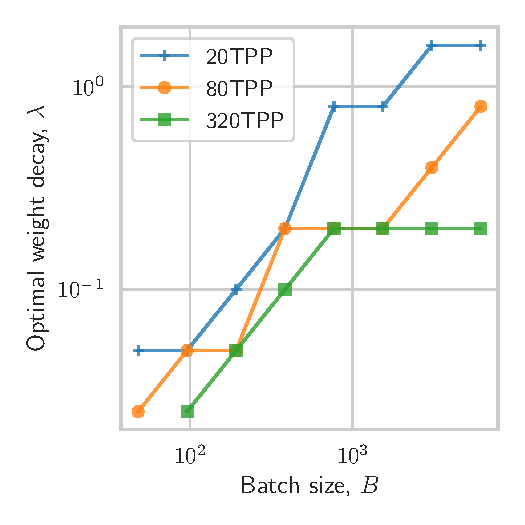
\includegraphics[trim={0.3cm 0.4cm 0.3cm 0.3cm}, clip, width=\linewidth]{pdffigs/batchwise_wds.111M.pdf}
    \caption{111M scale}
    \label{fig:more_wd_scaling_111M}
  \end{subfigure}
  \hfill %
  \begin{subfigure}[b]{\appendixwidth\textwidth}
    \centering
    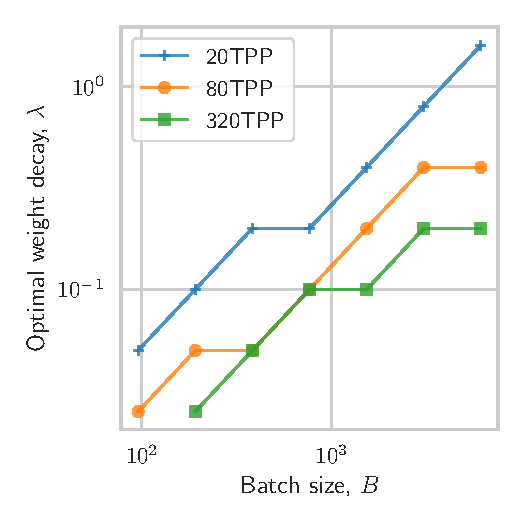
\includegraphics[trim={0.3cm 0.4cm 0.3cm 0.3cm}, clip, width=\linewidth]{pdffigs/batchwise_wds.266M.pdf}
    \caption{266M scale}
    \label{fig:more_wd_scaling_266M}
  \end{subfigure}
  \begin{subfigure}[b]{\appendixwidth\textwidth}
    \centering
    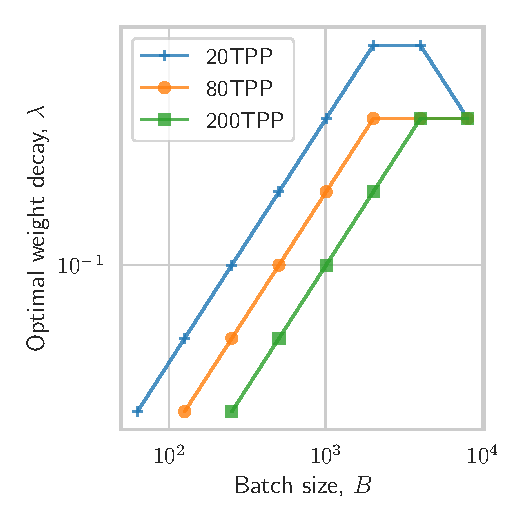
\includegraphics[trim={0.3cm 0.4cm 0.3cm 0.3cm}, clip, width=\linewidth]{pdffigs/batchwise_wds.617M.pdf}
    \caption{610M scale}
    \label{fig:more_wd_scaling_617M}
  \end{subfigure}
  \hfill %
  \begin{subfigure}[b]{\appendixwidth\textwidth}
    \centering
    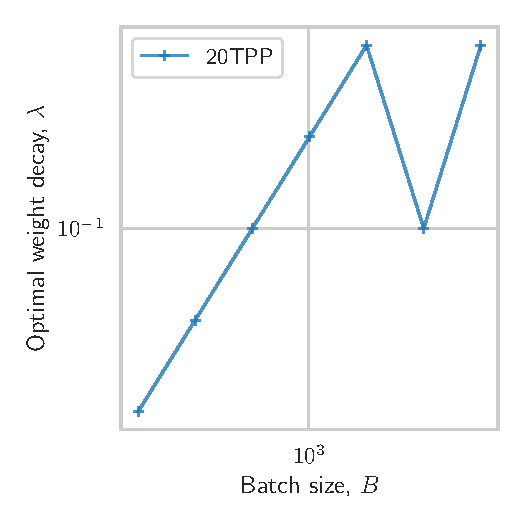
\includegraphics[trim={0.3cm 0.4cm 0.3cm 0.3cm}, clip, width=\linewidth]{pdffigs/batchwise_wds.1.7B.pdf}
    \caption{1.7B scale}
    \label{fig:more_wd_scaling_1_7B}
  \end{subfigure}
  \caption{\textbf{Optimal weight decay scaling with $B$}: The optimal
    weight decay increases linearly over small batch sizes---until
    $B > \cbs$.
    \label{fig:more_wd_scaling}}
\end{figure*}


\cref{fig:more_wd_scaling} shows how optimal $\lambda$ changes across
$B$, for all of the model scales and TPP levels where we did
hyperparameter sweeps.
%
There is a strong linear relationship between $\lambda$ and $B$ over
the smaller batch sizes $B < \bcrit$, with optimal $\lambda$
eventually plateauing (or decreasing).
%
Note the standard use of
$\lambda$=0.1~\citep{hoffmann2022empirical,brown2020language,almazrouei2023falcon,alephalpha2024introducing}
is only optimal at specific $B$, and this $B$ changes with TPP\@.

% This agrees with recent work showing that $\eta$ decreases when $B >
%\cbs$, when using the Adam
%optimizer~\citep{li2024surge,filatov2024time}.  Could the transition
%between linear scaling and no-further-scaling really be what's
%driving the square-root scaling rules discussed in related work?

\subsection{Additional details on $\tepoch$ fitting}\label{sec:appendix_tepoch_fitting}

\renewcommand{\algorithmiccomment}[1]{$\triangleright$ #1}
\begin{algorithm}[t]
  \caption{Generating the optimal $\tepoch$ power law}
  \label{alg:tepoch_fitting}
  \begin{algorithmic}
    \small
    \STATE {\bfseries Input:} small batch size $B$, optimal per-$N$ learning rates $\eta$ 
    \STATE Initialize $\tepochPoints = [$ $]$
    \FOR{$N$ {\bfseries in} $\modelScales$}  % N
      \FOR{$D$ {\bfseries in} $10N, 20N, 80N, 320N, ...$} % D
        \STATE Reset $\lossPoints = [$ $]$
        \FOR{$\lambda$ {\bfseries in} $\lambdaRange$} % lambda
          \STATE Train $\LLM(N,D,B,\lambda,\eta)$, get validation loss $L'$
          \STATE $\tepoch = \nicefrac{B}{\eta \lambda D}$
          \STATE $\lossPoints[\tepoch] = L'$
        \ENDFOR % L
        \STATE $\tepochopt = \argmin_{\tepoch}(\lossPoints)$
        \STATE $\tepochPoints.add( \langle \tpp$=$\nicefrac{D}{N}, \tepochopt \rangle )$
      \ENDFOR % D
    \ENDFOR % N
    \STATE Fit $\ctepochalg$, $\mtepochalg$ for $\tepochopt = {\ctepochalg} \tpp^{\mtepochalg}$ on $\tepochPoints$
  \end{algorithmic}
\end{algorithm}


We now describe how we obtained the optimal $\tema$ values at specific
model scales and TPP ratios.
%
Rather than taking the empirical minimum loss, we fit a parabola to
the $\langle \mathit{L}, \tepoch \rangle$ points in log space and took
the analytic minimum of the parabola.  If we have multiple loss values
at the same $\tepoch$ (e.g., our data for a single scale and TPP
comprises multiple different batch sizes), we only kept the lowest
loss points at each $\tepoch$ prior to parabola fitting.
%
We used validation loss on the held-out validation set.
%
For our $\tepoch$ calculations, we input $B$ in units of \emph{tokens}
(in contrast to the \emph{output} of our reported $\bopt$ and $\bcrit$
scaling laws, which we report in units of sequences, of 2048 tokens).
%
\cref{alg:tepoch_fitting} sketches the full procedure for generating
the $\tepoch$ power law (\cref{eq:tepoch_scaling}).
%
% Implied by taking the best ones?
%Note we are collecting $\tepoch$ here for runs where $B < \cbs$.

\subsection{Relationship to prior power laws}

\subsubsection{Relationship to $\etaopt$ scaling laws in dataset size, $D$}\label{sec:eta_scaling}

Both \citet{shen2024power} and \citet{bjorck2024scaling} propose
scaling laws for the optimal learning rate, $\etaopt$, as a power law
in the amount of data, $D$:
\begin{equation*}
  \etaopt = B \cdot \cetad \cdot D^{\metad}
\end{equation*}
We now discuss how this power law also follows from the power law of
$\tepochopt$ in TPP\@.  By \cref{eq:tepoch_scaling}, we have:
\begin{align*}
  \tepochopt(\tpp) &= {\ctepoch} \cdot \tpp^{\mtepoch} \\
  &= {\ctepoch} \cdot \left( \frac{D}{N} \right)^{\mtepoch}
\end{align*}
Substituting in the definition of $\tepoch$ (\cref{eq:tepoch}), and
assuming $\lambda$, $B$, and $N$ are
fixed,\footnote{\citet{bjorck2024scaling}\ use a fixed
$\lambda$=$0.1$, a fixed batch size of 0.5M tokens (for most of their
experiments), and fit scaling laws separately at different model sizes
(except in their Section~4).  \citet{shen2024power}\ use $\mup$ to
adjust the LR for different model scales, so the derivation applies at
any particular $N$; they do not report which optimizer is used nor any
of its settings.} this implies $\etaopt$ will scale as:
\begin{align}\label{eq:etaopt_equivalence}
  \frac{B}{\etaopt\lambda D} &= {\ctepoch} \cdot \frac{D^{\mtepoch}}{N^{\mtepoch}} \notag \\
  \Rightarrow \etaopt &= B \left( \frac{N^{\mtepoch}}{\lambda \cdot \ctepoch} \right) D^{-(\mtepoch + 1)} \notag \\
  &= B \cdot \cetad \cdot D^{\metad}
\end{align}
\begin{equation*}
  \text{where} \quad 
  \cetad = \frac{N^{\mtepoch}}{\lambda \cdot \ctepoch}
  \quad \text{and} \quad
  \metad = -(\mtepoch + 1)
\end{equation*}
\cref{eq:etaopt_equivalence} is exactly the form of the power law used
in \citet{shen2024power}, and explains the results across batch sizes
seen in \citet{bjorck2024scaling}, as discussed in
\cref{sec:tema_results}.

\paragraph{Comparison to fit in Power Scheduler~\citep{shen2024power}}\label{sec:appendix_power_scheduler}

Given $\cetad = \frac{N^{\mtepoch}}{\lambda \cdot \ctepoch}$ and $\metad =
-(\mtepoch + 1)$, we can use these formulas to compare our fit
coefficients to those in \citet{shen2024power}.

In \citet{shen2024power}, they find $\metad = -0.51$.
%
In our case, $\mtepoch = -0.520$, and therefore $\metad = -0.48$, which
is quite similar.

Comparing our $\cetad$ to their $\cetad$ ($= 4.6$) is a bit less
straightforward.  First of all, \citet{shen2024power} inputs $B$
in sequences (of length 4096).  We thus convert to the scale of our
coefficient by dividing by their sequence length, obtaining $\cetad =
0.0011$.
%
Secondly, the power law of \citet{shen2024power}\ is actually for
the \emph{base} $\mup$ learning rate $\hateta$, while our derivation
above assumes the adjusted (final) learning rate $\eta$
(\cref{sec:mup}).

Let us first compare $\cetad$ coefficients at the proxy-model scale,
i.e., where $\eta = \hateta$.
%
If we were to use a 28M-parameter proxy model, and a default
$\lambda$=0.1 (and using our fit values of $\ctepoch=1.084$ and
$\mtepoch=-0.527$), then, by $\cetad = \frac{N^{\mtepoch}}{\lambda
  \ctepoch}$, our $\cetad$ would also equal $0.0011$.

Now we consider how our coefficient varies when $N$ scales.  To
convert our $\eta$ scaling law into one for the base $\hateta$, we can
instead use $\cetad = \frac{N^{\mtepoch}}{\lambda \cdot \rho \cdot \ctepoch}$, where $\rho = P/W$, $P$ is the width of the proxy model,
and $W$ is the width of the target model.
%
The width also affects the number of parameters, $N$, and hence the
term $N^{\mtepoch}$.  In Transformers, $N$ scales roughly as $N
\propto L W^2$, where $L$ is the model depth and $W$ is the model
width.  If we round the fitted exponent to $\mtepoch \approx -0.5$,
and substitute the value $\rho \propto 1/W$ into the denominator, we
therefore have:
\begin{align*}
  \cetad &= \frac{N^{\mtepoch}}{\lambda \rho \ctepoch} \\
  &\propto \frac{N^{-0.5}}{\frac{1}{W}} \\
  &\propto {(L W^2)}^{-0.5}W \\
  &\propto {L}^{-0.5}{(W^2)}^{-0.5}W \\
  &\propto {L}^{-0.5}
\end{align*}
which is invariant to changes in $W$---i.e., the $\mup$ adjustment
cancels out the model scaling in width.
%
So, if we only scale $W$, $\tema$ scaling would stay in agreement with
the Power Scheduler recipe, but if we increase depth, $\tema$ scaling
would decrease $\eta$ proportional to $\nicefrac{1}{\sqrt{L}}$ in a
manner that is not accounted for in \citet{shen2024power}.

The key point is that the scaling law used by
\citet{shen2024power}\ is valid, indeed, has similar fitted exponents,
to what would be predicted by the $\tepochopt$ scaling law---but in a
specific context only (small models, or models only scaling in width).
%
Moreover, we have shown it may be less effective to adjust $\eta$ in
order to optimize $\tepoch$ (as these approaches implicitly do); we
obtained superior results by instead adjusting $\lambda$.  By
considering $\eta$, $\lambda$, and $B$ holistically, our scaling laws
are a superset of these laws for $\etaopt$, as well as other laws that
we discuss further presently.

\subsubsection{Relationship to $\etaopt$ scaling laws in model size, $N$}\label{sec:appendix_etaopt}

\cref{sec:tema_methods} gave our recipe for tuning hyperparameters,
for an arbitrary $N$, $D$, and $B$ setting.  Here we advocated setting
peak $\eta$ to the $\mup$-adjusted learning rate (where the base
learning rate comes from proxy-tuning).
%
Rather than further adjusting this LR based on the dataset size or
batch size, we argued for instead adjusting $\lambda$ so that
$\tepoch$ is tuned to its optimal value.  Based on both theory, and
our empirical findings comparing tuning $\eta$ to tuning $\lambda$, we
believe that using $\mup$ to scale $\etaopt$ with model width is
sufficient for well-tuned models.
%
That is, the \emph{theoretical} scaling law for $\etaopt$ (in model
width), given by $\mup$, is sufficient for good performance.
%
We discuss this perspective further in this section, specifically how
the $\mup$ scaling law can explain recent work in \emph{empirical}
$\etaopt$ power laws.

As noted in \cref{sec:mup}, when using $\mup$, a base $\eta$ is tuned
on a small proxy model, and then scaled depending on the width of the
target model.  Let $W$ be the width of the target model, and let $P$
be the width of the proxy model.  $\mup$ prescribes scaling the
optimal base learning rate, $\hatetaopt$, down to $\etaopt =
\rho\hatetaopt$, where $\rho=P/W$.  That is, $\etaopt =
P\hatetaopt/W$.
%
As models grow in size, $P$ and $\hatetaopt$ do not change, so
$\etaopt$ will scale $\propto 1/W$.
%
\citet[Figure~2]{dey2024practitioner} show that, indeed, a range of
LLMs from the GPT, Llama, and DeepMind series are roughly following a
scaling law where their chosen learning rate, $\eta$ is following
$\eta \propto {1}/{W}$.
%
In other words, if one were to build a scaling law for $\etaopt$ based
on published LLM settings, it would roughly obey the $\mup$
theoretical scaling law.

Furthermore, we can develop a scaling law for $\etaopt$ in model size,
$N$, using $\mup$, and show that it matches a recent empirical scaling
law by \citet{porian2024resolving}.  The number of model parameters in
any Transformer-based LLM scales roughly in the depth, $L$, and width,
$W$, as $N \propto L W^2$.  If we assume that we maintain a fixed
width-to-depth ratio, i.e., $R = W/L$, or $L = W/R$, then we have $N
\propto W^3$, or $W \propto N^{1/3}$.
%
Now, since $\mup$ prescribe scaling $\etaopt \propto W^{-1}$, then for
a fixed aspect ratio, $\etaopt \propto N^{-1/3}$.

Taking a very different approach, \citet{porian2024resolving}
developed an empirical scaling law for $\etaopt$ as a function of the
number of model parameters.  At each model scale, they trained with a
variety of batch sizes and learning rates, and found the optimal
settings of these hyperparameters.  All models were trained to 20
TPP\@.  They then fit a power law through the optimal LR settings, and
found that $\etaopt \propto N^{-1/3}$, exactly as would be expected if
one simply followed $\mup$.

As it provides a principled approach to scaling hyperparameters,
$\mup$ can adapt to scaling when aspect ratio is not fixed.  We
therefore advocate using $\mup$ to set $\etaopt$, rather than fitting
special $\etaopt$ power laws.
%
However, with regards to our overall approach, it does not actually
matter whether one uses the $\mup$ theoretical scaling law \emph{or}
an empirical one.  The key point is that these laws can be used to set
$\eta$ at a particular model scale, while the $\tepoch$ law should
further be used to set $\lambda$ depending on the $B$ or $D$ values.

%Both \citet{porian2024resolving} and \citet{bi2024deepseek} utilize
%joint scaling laws for $\eta$ and $B$.  The benefit of this approach
%is that $\eta$ can be tuned for early-stage training dynamics
%(maximizing movement from initial conditions, e.g., via $\mup$, the
%\emph{maximal} update parameterization), while $B$ simultaneously
%optimizes $\tepoch$.  The drawback, as mentioned in
%Section~\ref{sec:related} when discussing power laws for $\bopt$, is
%that if we rely on tuning $B$ to optimize $\tepoch$, we do not have
%flexibility to pick a batch size that optimizes the tradeoff between
%parallelism and compute efficiency.  We discuss batch size laws
%further in the following section.

\subsection{The EMA perspective and learning rate schedules}\label{sec:ema_lr}

To understand how the EMA view applies with a dynamic LR schedule, we
follow the discussion of \citet{bergsma2025straight}, who extended the
formulation in \citet{wang2024how}.
%
\citet{bergsma2025straight} consider EMAs with time-varying smoothing,
$\alpha_t \in [0, 1]$.  Letting $\alpha_1=1$ (i.e., $y_1=x_1$), they
express $y_t$ in terms of all inputs $x_t$:
\begin{eqnarray}\label{eqn:extended_ema}
  y_1 &=& \alpha_1 x_1  \notag, \\
  y_2 &=& (1 - \alpha_2) \alpha_1 x_1 + \alpha_2 x_2, \cdots  \notag \\
%  y_3 &=& (1 - \alpha_3) (1 - \alpha_2) \alpha_1 x_1 + (1 - \alpha_3) \alpha_2 x_2 + \alpha_3 x_3, \cdots \notag \\
%  &\cdots&  \notag \\
  y_t &=& \sum_{i=1}^t \left( \prod_{j=i+1}^{t} (1 - \alpha_j) \right) \alpha_i x_i
\end{eqnarray}

The EMA coefficient on each input is denoted $c_{t,i}$, where
%
\mbox{$c_{t,i} = \left( \prod_{j=i+1}^{t} (1 - \alpha_j) \right)
  \alpha_i$}.
%
In other words, $c_{t,i}$ reflects the contribution of input $x_i$ to
output $y_t$ at time $t$, such that
%
$y_t = \sum_{i=1}^t c_{t,i} x_i$.
%
Unlike a standard EMA with a fixed smoothing parameter, in this
extended EMA the coefficients need not decrease exponentially as $i$
decreases.  Indeed, any set of coefficients can be generated by some
particular smoothing schedule.

\begin{figure*}[t]
  \centering
  \begin{subfigure}[b]{0.32\textwidth}
    \centering
    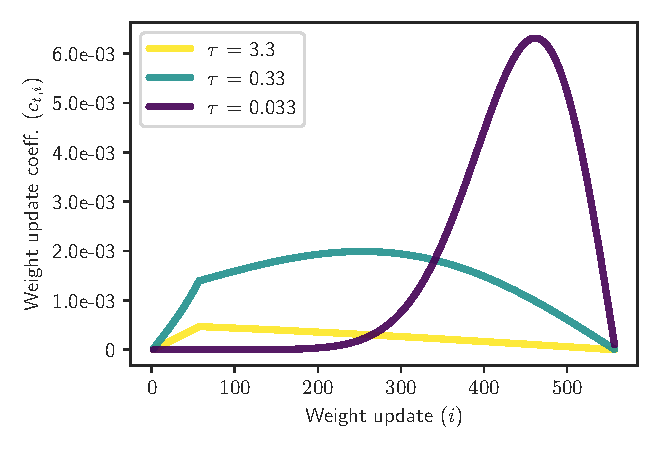
\includegraphics[trim={0.3cm 0.4cm 0.3cm 0.3cm}, clip, width=\linewidth]{pdffigs/111M.tepoch.linear.D2Z.WD=varies.0.2TPP.v2.pdf}
    \label{fig:emas_tepoch_2TPP}
    \caption{557 steps}
  \end{subfigure}
  \hfill
  \begin{subfigure}[b]{0.32\textwidth}
    \centering
    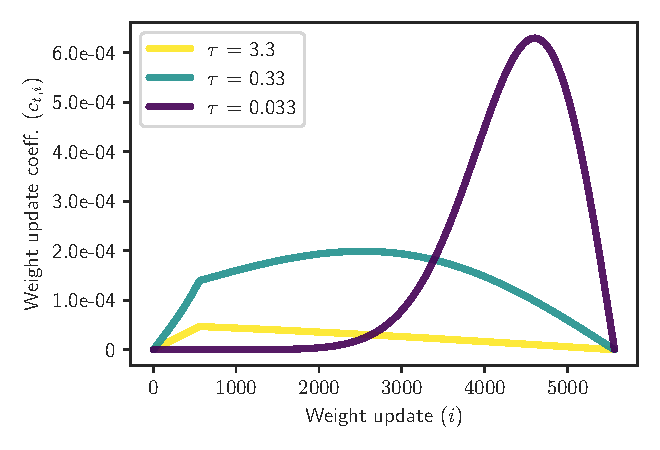
\includegraphics[trim={0.3cm 0.4cm 0.3cm 0.3cm}, clip, width=\linewidth]{pdffigs/111M.tepoch.linear.D2Z.WD=varies.0.20TPP.v2.pdf}
    \label{fig:emas_tepoch_20TPP}
    \caption{5568 steps}
  \end{subfigure}
  \hfill 
  \begin{subfigure}[b]{0.32\textwidth}
    \centering
    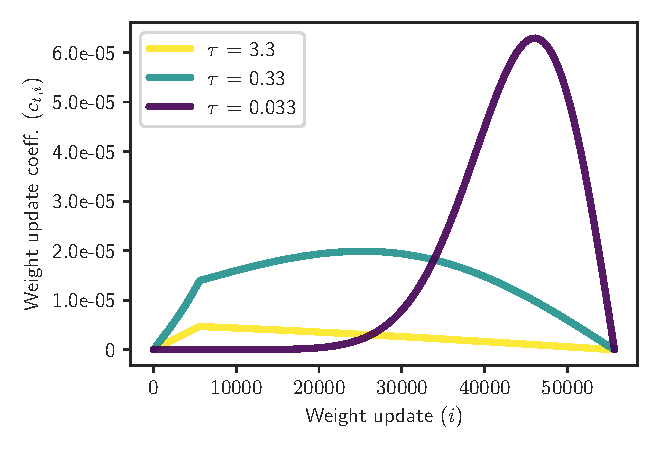
\includegraphics[trim={0.3cm 0.4cm 0.3cm 0.3cm}, clip, width=\linewidth]{pdffigs/111M.tepoch.linear.D2Z.WD=varies.0.200TPP.v2.pdf}
    \label{fig:emas_tepoch_200TPP}
    \caption{55680 steps}
  \end{subfigure}
  \caption{\textbf{$\tepoch$ is invariant to steps, with a learning
      rate decay schedule} (111M scale, proxy-tuned peak $\eta$ with
    linear decay-to-zero): Here we adjust weight decay, $\lambda$, in
    order to maintain $\tepoch$ at a constant value, decreasing
    $\lambda$ proportional to the increase in $S$.  Regardless of the
    total number of optimization steps, we see that the same $\tepoch$
    corresponds to the same \emph{shape} of the distribution of weight
    update coefficients (i.e., the same shape over the \emph{data},
    regardless of how the data is discretized in training).  For batch
    sizing, this means that if we use a constant $D$ but increase $B$
    by $K$$\times$ (decreasing $S$ by $K$$\times$), we will
    incorporate information across the {data} similarly---provided
    we use the same $\tepoch$.\label{fig:emas_tepoch}}
\end{figure*}


In terms of learning rate schedules for AdamW training, $\alpha_t =
\eta_t\lambda$ becomes the smoothing parameter at step $t$
(cf. \cref{sec:ema}).  The EMA itself, $y_t$, is the model parameters.
The EMA is over weight updates: a large coefficient $c_{t,i}$ means
the $i$th weight update contributes a lot to the EMA at step $t$.  The
EMA coefficients thus provide a more granular view of the contribution
timescale than $\tema$ alone.

We now study the question, how do the EMA coefficients change as the
step count changes?
%
We generated the $c_{t,i}$ coefficients for the linear decay-to-zero
LR schedule, and plot these coefficients at the final step (i.e.,
showing the contribution of weight updates to the final parameters).
%
We use the $\mup$-tuned and adjusted peak $\eta$, for 111M models.
%
The learning rate increases linearly to the peak for the first 10\% of
steps, then decreases from the peak to 0 for the remainder of steps.
We simulated three cases: where we take 557 steps, where we take 5568
steps, and where we take 55680 steps (5568 steps would be 20 TPP for a
111M model using $B$=192).
%
From the perspective of batch sizing, these different steps could be
achieved by decreasing the batch size twice by $10\times$.

We adjusted $\lambda$ for each step count in order to obtain the same
three specific $\tepoch$ values.  In \cref{fig:emas_tepoch}, we see
that the same $\tepoch$ implies the same \emph{shape} of coefficients
across the steps, and hence the same contribution over (normalized)
time.  That is, weight updates from the same portion of the training
data contribute equally to the final model parameters.\footnote{Note
we do not plot the initial coefficients $c_{t,0}$ here, but they are
equal across the scales for a given $\tepoch$, unlike the non-initial
coefficients, which reduce by $10\times$ as the number of steps
increases by $10\times$.  So a constant $\tepoch$ means both the same
contribution across the data, \emph{and} the same \emph{bias}
(dependence on initial weights).}

The key takeaway is that since $\tepoch$ is independent of the number
of steps, it theoretically provides a $B$-independent measure of the
AdamW timescale over weight updates, regardless of learning rate
schedule.
%
However, this equivalence for different $B$ breaks down when $B >
\cbs$ and weight updates themselves no longer contain linearly
$B\times$ the information of a single sample.

%\subsection{And EMA view of how $\tepoch$ changes with TPP}\label{sec:ema_tpp}
%
%TODO: draw the x-axis in ``proportion of steps'' and plot our fit
%values for TPP=5, TPP=10, TPP=20, TPP=80, TPP=320, TPP=1280.

\section{Scaling of $\bopt$ and $\bcrit$: additional details and results}

\subsection{Derivation of ``extra data'' \cref{eq:s_extra}}\label{sec:cbs_derivations}

% TOO COMPLICATED!
%It is worth noting that in \citet{mccandlish2018empirical}, the
%tradeoff equation (our \cref{eq:tradeoff}) is derived by averaging
%their Equation 2.7 over multiple optimization steps.  Their Equation
%2.7 gives the reduction in loss given a finite batch size of $B$ as a
%function of the maximum possible reduction in loss (with an infinite
%$B$) as 

%Something about how \cref{eq:tradeoff} itself arises from the
%per-step loss equation in~\citet{mccandlish2018empirical} (their
%equation 2.7).

\cref{eq:tradeoff} can be written as:
\begin{align*}
  \frac{D - \dmin}{\dmin} &= \frac{\smin}{S - \smin} \\
  \Rightarrow (D - \dmin)(S - \smin) &= \dmin \smin \\
  \Rightarrow D S - D \smin - S \dmin &= 0
\end{align*}
Given $B = {D}/{S}$, we can substitute in
$S={D}/{B}$ to get an equation in a single variable, from
which we can solve for $D$.
\begin{align*}
  \frac{D^2}{B} - D \smin - \frac{D \dmin}{B} &= 0 \\
  \Rightarrow D^2 - D B \smin - D \dmin &= 0 \\
  \Rightarrow D (D - B \smin - \dmin) &= 0 \\
  \Rightarrow D &= \dmin + B \smin
\end{align*}
Given $\cbs = {\dmin}/{\smin}$, we can substitute $\smin = {\dmin}/{\cbs}$ and obtain:
\begin{align*}
  \Rightarrow D &= \dmin + B \frac{\dmin}{\cbs} \\
  \Rightarrow D &= \dmin \left( 1 + \frac{B}{\cbs} \right)
\end{align*}

\subsection{Estimating $\cbs$}\label{sec:appendix_estimating_cbs}

We first provide some learnings from developing the $\cbs$ estimation
procedure.

First, regarding the functional form $L_{B}(D) = \irr + \dconst
D^{-\beta}$, we found that including the irreducible loss term $\irr$
was important for obtaining good fits.  $\irr$ conceptually represents
the Bayes risk \emph{plus} the minimum loss obtainable for a model of
size $N$ (i.e., the first two terms of \cref{eq:chinchilla}).
%
Second, only \emph{interpolated} points were reliable; we only compute
$\cbs$ for loss values where all points are between, or very near to,
curve fitting points.
%
Third, each power law should have at least $3$ points for fitting, in
order to capture the concavity of the scaling in $D$.
%
Finally, we sample our $B$ values logarithmically and, as in
\citet{mccandlish2018empirical}, perform our fits to
\cref{eq:tradeoff} in log space.

\begin{figure*}[t]
  \centering
  \begin{subfigure}[b]{\appendixwidth\textwidth}
    \centering
    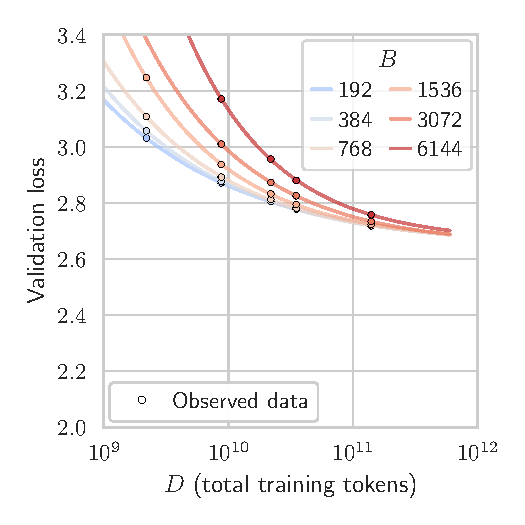
\includegraphics[trim={0.3cm 0.4cm 0.3cm 0.3cm}, clip, width=\linewidth]{pdffigs/241005.fitted_scale_law.gbs=multi.111M.pdf}
    \caption{111M scale}
    \label{fig:quad_cbs_111M}
  \end{subfigure}
  \hfill
  \begin{subfigure}[b]{\appendixwidth\textwidth}
    \centering
    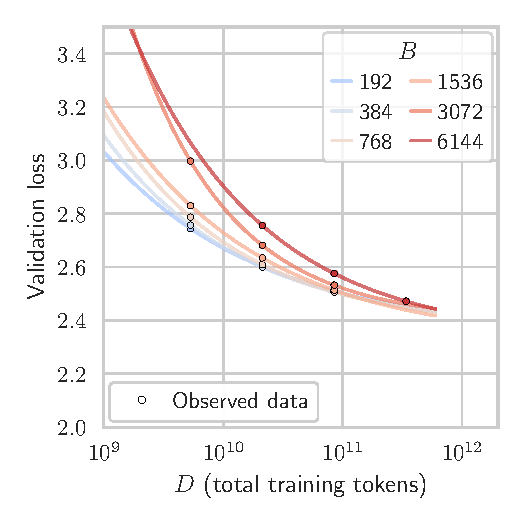
\includegraphics[trim={0.3cm 0.4cm 0.3cm 0.3cm}, clip, width=\linewidth]{pdffigs/241005.fitted_scale_law.gbs=multi.266M.pdf}
    \caption{266M scale}
    \label{fig:quad_cbs_266M}
  \end{subfigure}
  % Next row
  \begin{subfigure}[b]{\appendixwidth\textwidth}
    \centering
    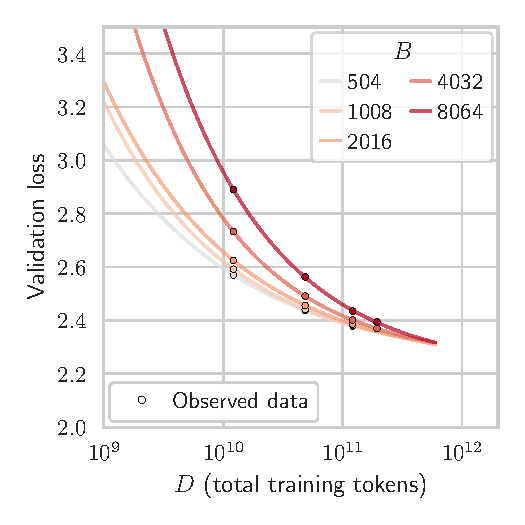
\includegraphics[trim={0.3cm 0.4cm 0.3cm 0.3cm}, clip, width=\linewidth]{pdffigs/241005.fitted_scale_law.gbs=multi.617M.pdf}
    \caption{610M scale}
    \label{fig:quad_cbs_617M}
  \end{subfigure}
  \hfill
  \begin{subfigure}[b]{\appendixwidth\textwidth}
    \centering
    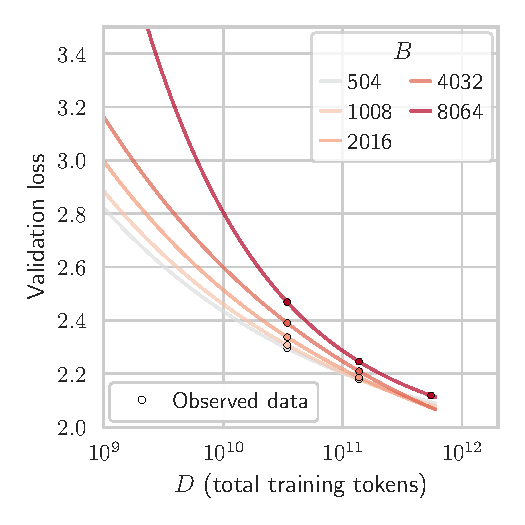
\includegraphics[trim={0.3cm 0.4cm 0.3cm 0.3cm}, clip, width=\linewidth]{pdffigs/241005.fitted_scale_law.gbs=multi.1.7B.pdf}
    \caption{1.7B scale}
    \label{fig:quad_cbs_1_7B}
  \end{subfigure}
  \caption{\textbf{Scaling laws in $D$ for computing $\cbs$}: Full set
    of $B$-specific power laws, for 111M to 1.7B scales, fitted after
    training models with different batch sizes, $B$, and dataset
    sizes, $D$, at each scale (empirical data from real training runs
    indicated by points).  From these power laws, we can compute the
    amount of data needed to reach any target loss, as illustrated in
    main paper \cref{fig:cbs_fitting}.\label{fig:quad_cbs_fitting}}
\end{figure*}


\cref{fig:quad_cbs_fitting} illustrates all the fit scaling laws for
the $\cbs$ experiments.  Notice that beyond the fitting points, the
curves may not predict behavior well.
%
In particular, we would expect all curves to eventually converge as
$D$ increases.  Because loss targets beyond the fitting points are
unreliable, we only compute $\cbs$ at loss targets where all the data
sizes can be estimated through interpolation.

\begin{figure*}[th]
  \centering
  \begin{subfigure}[b]{0.49\textwidth}
    \centering
    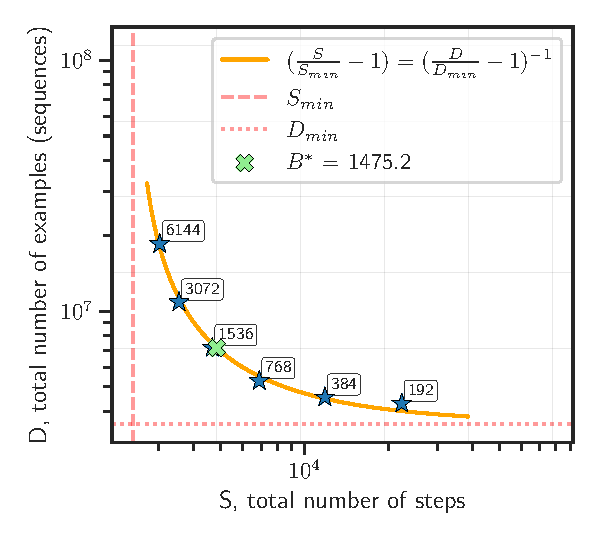
\includegraphics[trim={0.3cm 0.4cm 0.3cm 0.3cm}, clip, width=\linewidth]{pdffigs/loss_data.241005_batchsizes.111M.l=2.872.cbs.pdf}
    \caption{111M, loss=2.872}
    \label{fig:quad_cbs_fits_111M}
  \end{subfigure}
  \hfill
  \begin{subfigure}[b]{0.49\textwidth}
    \centering
    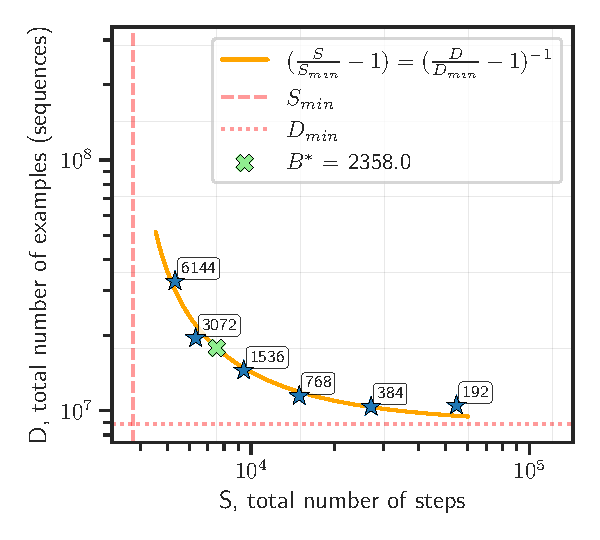
\includegraphics[trim={0.3cm 0.4cm 0.3cm 0.3cm}, clip, width=\linewidth]{pdffigs/loss_data.241005_batchsizes.266M.l=2.600.cbs.pdf}
    \caption{266M, loss=2.600}
    \label{fig:quad_cbs_fits_266M}
  \end{subfigure}
  % Next row
  \begin{subfigure}[b]{0.49\textwidth}
    \centering
    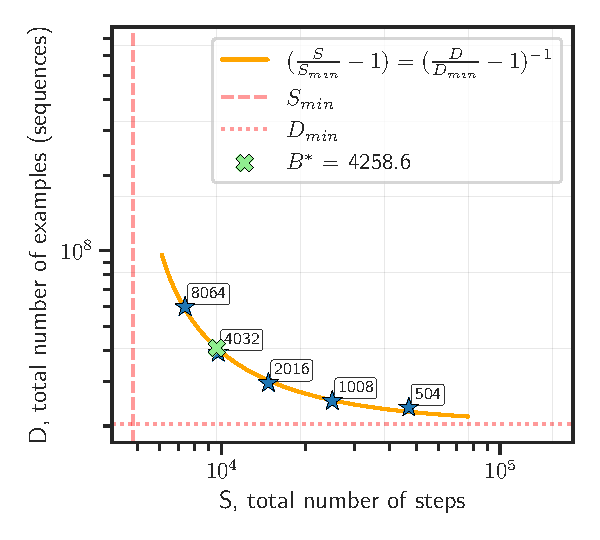
\includegraphics[trim={0.3cm 0.4cm 0.3cm 0.3cm}, clip, width=\linewidth]{pdffigs/loss_data.241005_batchsizes.610M.l=2.437.cbs.pdf}
    \caption{610M scale, loss=2.437}
    \label{fig:quad_cbs_fits_617M}
  \end{subfigure}
  \hfill
  \begin{subfigure}[b]{0.49\textwidth}
    \centering
    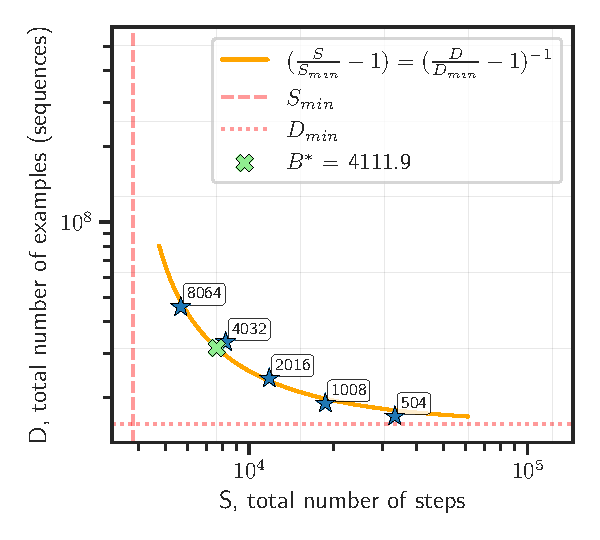
\includegraphics[trim={0.3cm 0.4cm 0.3cm 0.3cm}, clip, width=\linewidth]{pdffigs/loss_data.241005_batchsizes.1.7B.l=2.295.cbs.pdf}
    \caption{1.7B scale, loss=2.295}
    \label{fig:quad_cbs_fits_1_7B}
  \end{subfigure}
  \caption{\textbf{Example fits of trade-off \cref{eq:tradeoff}
      plotting $\smin$ and $\dmin$}: The empirical data has a good fit
    with \cref{eq:tradeoff} across model scales and loss targets.
    These estimates of $\cbs$ are used in fitting the $\cbs$-scaling
    power law
    (\cref{fig:hook} $\rightfig$).\label{fig:quad_cbs_fits}}
\end{figure*}


\cref{fig:quad_cbs_fits} shows the specific fits of \cref{eq:tradeoff}
at particular loss targets.  While \cref{eq:tradeoff} reflects the
data trend well over the given $B$ values, we consistently find that
points with very small $B$ do not approach $\dmin$.  We discussed this
observation further in \cref{sec:limitations}.

\renewcommand{\algorithmiccomment}[1]{$\triangleright$ #1}
\begin{algorithm}[tb]
  \caption{Generating the $\cbs$ power law}
  \label{alg:cbs_fitting}
  \begin{algorithmic}
    \small
    \STATE Initialize $\cbsPoints = [$ $]$
    \FOR{$N$ {\bfseries in} $\modelScales$}  % N
      \STATE \COMMENT{Fit $B$-specific (and $N$-specific) scaling laws, $L_{B}(D)$:}
      \FOR{$B$ {\bfseries in} $\batchSizes[N]$}  % B
        \STATE Reset $\scaleSet = [$ $]$
        \FOR{$D$ {\bfseries in} $10N, 20N, 80N, 320N, ...$} % D
          \STATE Train $\LLM(N,D,B)$, get validation loss $L'$
          \STATE $\scaleSet.add( \langle D,L' \rangle )$
        \ENDFOR % D
      \STATE Fit $\irr$, $\dconst$, $\beta$ for $L_{B}(D) = \irr + \dconst D^{-\beta}$ on $\scaleSet$
      \ENDFOR % B
      \STATE \COMMENT{Use $L_{B}(D)$ to estimate $\cbs$ at various loss values:}
      \FOR{$\hat{L}$ in $lossTargets[N]$} % L
        \STATE Reset $\tradeoffSet = [$ $]$
        \FOR{$B$ {\bfseries in} $\batchSizes[N]$} % B
          \STATE Get $\dinfer = L_{B}^{-1}(\hat{L}) = \left(\frac{\dconst}{\hat{L}-\irr}\right)^{\frac{1}{\beta}}$
          \STATE $\tradeoffSet.add( \langle \dinfer, S$=$\nicefrac{\dinfer}{B} \rangle )$
        \ENDFOR % B
        \STATE Fit $\dmin$, $\smin$ for \cref{eq:tradeoff} on $\tradeoffSet$
        \STATE $\cbs = \nicefrac{\dmin}{\smin}$
        \STATE $\cbsPoints.add( \langle \dmin, \cbs \rangle )$
      \ENDFOR % L
    \ENDFOR % N
    \STATE Fit $\ccbsalg$, $\mcbsalg$ for $\cbs = {\ccbsalg} (\dmin)^{\mcbsalg}$ on $\cbsPoints$
  \end{algorithmic}
\end{algorithm}


Finally, for clarity, we provide \cref{alg:cbs_fitting}, which gives
the detailed approach to generating the $\cbs$ power law in procedural
form.

\subsection{Estimating $\cbs$ for the 3.3B model}

To obtain an estimate of $\bcrit$ for the 3.3B model (shown in
\cref{fig:hook}, $\rightfig$), it was not feasible to apply our full
$\cbs$ fitting procedure at this scale (i.e., fitting $B$-specific
loss power-laws, etc.).
%
Instead, we estimated $\bcrit$ based on two $B$, $\dmin$ pairs.
%
That is, (based on an initial estimate of $\bcrit$) we trained a 3.3B
model to 23TPP with $B$=2016 and got a loss of 2.1688, and a separate
model to 30TPP with $B$=4032, obtaining a loss of 2.1695.
%
Given these losses are very close, these two models should have the
same $\bcrit$ and thus same $\dmin$.

We solve for this $\bcrit$ as follows.  Let $B_2 = 4032$ and $B_1 = 2016$.  By \cref{eq:s_extra}:
\begin{align*}
  D_2 &= \dmin(1 + B_2/\bcrit), \text{and} \\
  D_1 &= \dmin(1 + B_1/\bcrit)
\end{align*}
Let $r = D_2/D_1$ (i.e., 30/23 in this case).  If we divide the above
equations, and solve for $\bcrit$, we find:
\begin{align*}
  \bcrit &= \frac{B_2 - r B_1}{r - 1}
\end{align*}
Plugging in our values of $r$, $B_1$, and $B_2$, we obtain an
estimated $\bcrit$ of 4610, corresponding to a $\dmin$ of
approximately 16 TPP\@.

\subsection{$\cbs$ scaling in loss}\label{sec:appendix_loss_scaling}

\cref{fig:related} ($\middlefig$) shows that $\cbs$ is clearly not a
power law in loss, as proposed in prior
work~\citep{mccandlish2018empirical,kaplan2020scaling,li2024surge}.
However, if we only consider points with the same TPP, there does
appear to be somewhat of a power-law relationship.  In fact, this is
implied by $\cbs$ being a power law in $D$, along with the (standard)
assumption that loss scales similarly in $N$ and $D$.

Specifically, let $\hatr = {D}/{N}$ be the fixed TPP ratio.
Therefore, $N = {D}/{\hatr}$.  Assuming loss follows
\cref{eq:chinchilla}, we have:
\begin{align*}
L(N,D) &= E + \nconst N^{-\alpha} + \dconst D^{-\beta} \\
       &= E + \nconst \left( \frac{D}{\hatr} \right)^{-\alpha} + \dconst D^{-\beta} \\
       &= E + \nconst \hatr^{\alpha} D^{-\alpha} + \dconst D^{-\beta}
\end{align*}
Now, if $\alpha \approx \beta$, as is commonly
accepted~\citep{hoffmann2022empirical,besiroglu2024chinchilla,krajewski2024scaling,porian2024resolving,gadre2024language}, we have:
\begin{align*}
  L(D) &= E + (\nconst \hatr^{\alpha} + \dconst) D^{-\alpha} \\
   &= E + \kconst D^{-\alpha}
\end{align*}
where $\kconst = \nconst \hatr^{\alpha} + \dconst$ is a constant.  In
other words, at a fixed TPP, loss is a power law in data.  Given
$\bcrit$ is also fundamentally a power law in data, then by the
transitivity of power law relationships, $\cbs$ is also a power law in
loss in this context.  This relationship can also be derived by
expressing the $D$ in \cref{eq:cbs_scaling} as a power law in $\cbs$,
and substituting into $E + K D^{-\alpha}$.

\subsection{Weight decay affects $B$ scaling laws}\label{sec:app_wd_affects_b}

\begin{table}[]
  \centering
  \caption{Different $\lambda$ settings systematically affect fitted
    power laws for $\bopt$, and result in poorer fit quality (lower
    $\Rtwo$).  Fitted parameters change with $\lambda$ and
    consequently projected $\bopt$ values (in sequences) for different
    token budgets $D$.\label{tab:wd_bopt}}
  \begin{tabular}{@{}llllll@{}}
    \toprule
    Weight decay          & Scaling law                & $\Rtwo$ & D=1e10          & D=1e11          & D=1e12          \\ \midrule
    0.4                   & $\bopt = 0.0006 D^{0.607}$ & 0.706  & 587             & 2377            & 9615            \\
    0.2                   & $\bopt = 0.0012 D^{0.543}$ & 0.926  & 323             & 1128            & 3937            \\
    0.1                   & $\bopt = 0.0123 D^{0.429}$ & 0.972  & 240             & 644             & 1729            \\
    0.05                  & $\bopt = 0.384 D^{0.270}$  & 0.689  & 192             & 358             & 667             \\
    0.025                 & $\bopt = 10.3 D^{0.120}$   & 0.161  & 163             & 215             & 284             \\
    \emph{Tuned}          & $\bopt = 0.0306 D^{0.383}$ & \emph{0.984} & \emph{207}      & \emph{500}      & \emph{1207}     \\ \bottomrule
  \end{tabular}
\end{table}


\paragraph{Weight decay affects scaling of $\bopt$.}

\cref{tab:wd_bopt} illustrates how fixing $\lambda$ at different
values alters the fitted $\bopt$ power law. Larger $\lambda$
systematically yields larger $\bopt$ and poorer fit quality
(lower~$\Rtwo$). When $\lambda$ is fixed, the batch size that
minimizes loss is only a \emph{conditional optimum} (we denote it as
$\boptcond$) because it compensates for suboptimal
timescales~$\tema$ rather than representing the globally
tuned $\bopt$ obtained when $\lambda$ is optimized jointly.

The degraded $\Rtwo$ values arise because a fixed $\lambda$ forces $B$
to balance two partially competing goals: (1)~maintaining a good
$\tema$ value, and (2)~remaining below $\bcrit$ to avoid gradient
redundancy. A simple power law cannot capture this coupled behavior.

From the relation $\tema = B/(\eta\lambda D)$ and the empirical
scaling $\temaopt \propto (\nicefrac{D}{N})^{m}$
(\cref{eq:tepoch_scaling}), one can derive that, for constant $\eta$,
$\lambda$, and $N$, the batch size preserving $\temaopt$ should scale
as $B \propto D^{m+1}$ (with $m+1\!\approx\!0.47$ for our data). The
exponents in \cref{tab:wd_bopt}, however, deviate from~0.47. For
small~$D$ and large~$\lambda$, the $B$ that preserves $\temaopt$ lies
near or above $\bcrit$, yielding worse loss due to gradient
redundancy.  This means $\boptcond$ is artificially lower for small
$D$ values. Since $\boptcond$ is affected differently for different
$D$, the scaling law slope is distorted (in this case,
increased). Analogous issues disrupt $\boptcond$ for small $\lambda$.
These distortions reduce~$\Rtwo$ and impair generalization to
large-scale training. When $\lambda$ is tuned, this confound is
removed, and the resulting $\bopt$ law aligns cleanly with the
expected~$D^{0.4}$ scaling.

\paragraph{Weight decay affects scaling of $\bcrit$.}

A similar confound arises for~$\bcrit$. Fixing $\lambda$ causes
deviations from $\temaopt$ to mingle with true gradient-redundancy
effects.
%
At 111M scale and a target loss of~3.03, e.g., larger batches perform
worse solely because $\tema$ drifts from its optimal value, reducing
the fitted $\bcrit$ from~867 (tuned~$\lambda$) to~707
(fixed~$\lambda{=}0.1$).
%
At other loss targets, $\bcrit$ is less affected. Since
the estimated $\bcrit$ is affected differently at different scales,
the slope of the $\bcrit$ scaling law is again artificially
distorted. $\bcrit$ will appear to increase faster than $D^{0.5}$, and
projections to larger scales will be inaccurate.
%
In contrast, tuning~$\lambda$ isolates gradient-redundancy effects,
yielding a stable~$D^{0.5}$ relation that generalizes across scales.
